\documentclass[conference]{IEEEtran}
\IEEEoverridecommandlockouts

\usepackage[utf8]{inputenc}
\usepackage[T1]{fontenc}
\usepackage{amsmath,amssymb,amsfonts}
\usepackage{graphicx}
\usepackage{cite}
\usepackage{booktabs}
\usepackage{array}
\usepackage{url}

% Configure graphics search path for publication assets
\graphicspath{{../literature_survey/13_ablation_study/figures/}{research/literature_survey/13_ablation_study/figures/}}

\title{Turn-Aware Search and Road-Impedance Modelling for Two-Wheeler Routing in Urban Road Networks}

\author{
\IEEEauthorblockN{Anirudh R}
\IEEEauthorblockA{\textit{Department of Computer Science and Engineering} \\
\textit{BNM Institute of Technology}\\
Bengaluru, India \\
anirudhraju7@gmail.com}
\and
\IEEEauthorblockN{Shwetha M D}
\IEEEauthorblockA{\textit{Department of Computer Science and Engineering} \\
\textit{BNM Institute of Technology}\\
Bengaluru, India \\
shwetha.0116@gmail.com}
\and
\IEEEauthorblockN{Vikhyath K B}
\IEEEauthorblockA{\textit{Department of Computer Science and Engineering} \\
\textit{BNM Institute of Technology}\\
Bengaluru, India \\
vikhyathkb@bnmit.in}
\and
\IEEEauthorblockN{Akshath G}
\IEEEauthorblockA{\textit{Department of Computer Science and Engineering} \\
\textit{BNM Institute of Technology}\\
Bengaluru, India \\
23cse167@bnmit.in}
\and
\IEEEauthorblockN{A Nikhil Kumar}
\IEEEauthorblockA{\textit{Department of Computer Science and Engineering} \\
\textit{BNM Institute of Technology}\\
Bengaluru, India \\
23cse100@bnmit.in}
\and
\IEEEauthorblockN{Chiranandan T M}
\IEEEauthorblockA{\textit{Department of Computer Science and Engineering} \\
\textit{BNM Institute of Technology}\\
Bengaluru, India \\
23cse186@bnmit.in}
}

\begin{document}

\maketitle

\begin{abstract}
Conventional shortest-path routing on vertex-based road graphs does not inherently account for arrival heading when evaluating successive road segments. This limits its ability to represent turn-dependent routing costs and vehicle-specific road impedance within a unified search formulation. This paper presents a two-wheeler-oriented routing approach that combines state-expanded $A^*$ search with road-class impedance modelling. The search represents states as directed edge states $s=(u,v)$ and incorporates discrete angular penalties during edge relaxation. Road segments are assigned class-dependent impedance weights, with a $0.80$ override for qualifying grade-separated main-road segments. When composite edge multipliers satisfy $\mu(e) \ge 0.80$ and turn penalties are nonnegative, we establish the admissibility and consistency of a Haversine heuristic scaled by $0.80$. The approach is evaluated on 25 origin--destination corridors using a Bengaluru road network containing 744,216 directed edges. Compared with turn-unaware state-expanded routing (A1), the turn-aware configuration (A0) reduces the mean number of sharp turns ($\ge 60^\circ$) by $34.1\%$ ($32.52$ to $21.44$ turns; Holm-adjusted $p=4.5\times 10^{-5}$). Relative to neutral road-class impedance (B1), the production impedance configuration (B0) reduces arterial exposure by $51.21$ percentage points ($65.05\%$ to $13.84\%$), with a $15.53\%$ increase in mean physical route distance ($7.65$ vs. $6.62\text{ km}$). These results demonstrate the measurable effects of incorporating heading-dependent turn costs and road-class impedance into urban two-wheeler routing.
\end{abstract}

\begin{IEEEkeywords}
Two-wheeler routing, state-expanded search, turn penalties, shortest path algorithms, road impedance modeling, heuristic admissibility, urban transportation networks.
\end{IEEEkeywords}

\section{Introduction}

Urban road transport in Indian metropolitan areas is characterized by a dominant share of motorized two-wheelers, which experience distinct physical and operational friction compared to passenger cars \cite{promraksa2022lane,kotagi2020modeling}. In dense urban environments such as Bengaluru, riders routinely navigate complex topological networks characterized by high intersection densities, frequent grade changes, and acute-angle maneuvers. Standard commercial mapping services prioritize passenger automobiles, employing routing metrics that omit vehicle-specific physical impedance and turn-induced effort \cite{kumar2025realtime}. Consequently, algorithms optimized for four-wheeled vehicular travel frequently route two-wheelers through high-stress arterial corridors or recommend high-frequency turning sequences that impose disproportionate physical friction on riders.

Standard vehicular routing engines evaluate road networks using link travel time or distance costs evaluated at individual graph vertices \cite{luxen2011realtime}. While computationally efficient, this node-centric formulation cannot directly model turning movements because the legality and impedance of traversing an outbound edge $(v, w)$ depend strictly on the inbound trajectory $(u, v)$ \cite{das2019modeling,winter2002modeling}. Overcoming this limitation requires state-expanded search spaces, where graph states represent directed edge transitions $s=(u, v)$ rather than isolated physical intersections \cite{kirby1969minimum}.

Incorporating turn costs into shortest-path search requires expanding the network representation, as turn penalties depend fundamentally on the inbound approach angle and outbound departure heading \cite{winter2002modeling}. Classic edge-expanded graph formulations associate states with directed links, expanding vertex $|V|$ into edge $|E|$ states \cite{kirby1969minimum}. Modern contraction hierarchies (CH) \cite{geisberger2011efficient} and Customizable Contraction Hierarchies (CCH) \cite{bast2016route} accommodate turn costs during offline contraction phases. However, in heterogeneous urban networks where edge costs require multi-criteria evaluation---such as road hierarchy, surface penalties, and topological modifiers---preprocessing times and shortcut complexities increase substantially \cite{bast2016route}.

In two-wheeler routing, road classification is an essential determinant of rider stress and physical friction. Motorcyclists and scooter riders exhibit distinct spatial choice behaviors, frequently trading marginal distance increases for reduced exposure to high-speed arterial traffic or congested conflict zones \cite{fadilah2024identifying,asvial2020entropy}. Existing platforms that apply uniform distance or free-flow velocity metrics fail to capture this operational dichotomy. By failing to integrate road-class impedance directly into the cost objective, conventional route guidance channels two-wheelers into major thoroughfares where vehicular speed differentials heighten collision risks.

This paper proposes a two-wheeler routing framework combining state-expanded, turn-aware $A^*$ search with road-class-dependent impedance modeling. The search space is defined over directed edge transitions $s=(u, v)$, eliminating the need to construct explicit line graphs while supporting exact angular penalty computation during edge relaxation. Road segments are weighted by vehicle-specific impedance multipliers, with a $0.80$ override for qualifying grade-separated main-road segments. We establish the conditional admissibility and consistency of a Haversine heuristic scaled by $0.80$, proving exact optimality under non-negative turn penalties when all edge multipliers satisfy $\mu(e) \ge 0.80$ \cite{hart1968formal}. Evaluated across 25 real-world commute corridors in Bengaluru, the turn-aware framework ($A_0$) reduces sharp turning maneuvers ($\ge 60^\circ$) by $34.1\%$ relative to turn-unaware state-expanded routing ($21.44$ vs. $32.52$ turns; Holm-adjusted $p = 4.5 \times 10^{-5}$). Furthermore, production impedance modeling ($B_0$) decreases arterial exposure by $51.21$ percentage points ($13.84\%$ vs. $65.05\%$) with a $15.53\%$ increase in physical route distance ($7.65\text{ km}$ vs. $6.62\text{ km}$).

The remainder of this paper is organized as follows: Section II surveys related work in state-expanded routing, turn-penalty formulations, and two-wheeler routing. Section III formalizes the urban road network, discrete turn-deflection penalties, and configured road impedance. Section IV presents the turn-aware $A^*$ search algorithm, proves conditional heuristic admissibility and consistency, and establishes computational complexity bounds. Section V details the empirical setup and 25-corridor corpus. Section VI presents ablation results, scalability metrics, and inferential hypothesis testing across Experiments A--D. Section VII concludes with limitations and directions for future research.

\section{Related Work}

\noindent\textbf{Shortest-Path Routing and Turn-Aware State Representations:} Early formulations of turn penalties in transit and road networks established that turning delays cannot be modeled as independent vertex costs without expanding the network representation \cite{kirby1969minimum}. Winter demonstrated that modeling turn-dependent travel costs requires directed edge-to-edge transitions rather than simple node-to-node connectivity, formalizing line graphs and dual-graph representations for turn-aware search \cite{winter2002modeling}. While line-graph expansion preserves standard shortest-path algorithms, it increases graph cardinality by expanding vertices into edges $|E|$ and edges into valid turning movements, substantially increasing memory footprint on dense urban networks.

\noindent\textbf{Hierarchical Routing and Metric Customization:} Modern production routing engines achieve sub-millisecond query performance on continental-scale graphs using Contraction Hierarchies (CH) \cite{geisberger2011efficient} and Customizable Contraction Hierarchies (CCH) \cite{bast2016route,delling2017customizable}. Geisberger and Vetter extended node contraction to incorporate turn costs through node-expansion techniques and turn-aware node ordering \cite{geisberger2011efficient}. However, customizable hierarchical techniques decouple metric customization from preprocessing, requiring re-customization phases whenever cost functions or vehicle-specific profile weights change. On dynamic urban street networks with heterogeneous vehicle constraints, maintaining hierarchical speedup indexes introduces operational complexity.

\noindent\textbf{Two-Wheeler Trajectory Analysis and Rider Preference:} Two-wheeler navigation operates under mixed-traffic conditions characterized by vehicle speed dispersion \cite{kotagi2020modeling} and queue lane-filtering \cite{promraksa2022lane}. In Ninh Ki\^{e}u District, C\^{a}n Th\textsubscript{o}, Vietnam, Fadilah et al. \cite{fadilah2024identifying} used stated-preference modelling and microscopic simulation to examine motorcycle route selection under traffic-information scenarios, reporting departures from static shortest-path assignments in the simulated results. For two-wheeler routing, Asvial et al. \cite{asvial2020entropy} evaluated route suitability by generating candidate paths without turn penalties and applying post-hoc Entropy-TOPSIS re-ranking. Rather than re-ranking candidate paths or modeling behavioral choice, we evaluate configured road impedance directly within graph search as an engineering heuristic, without asserting that configured multipliers represent calibrated rider preferences.

\noindent\textbf{Research Positioning and Synthesis:} Prior literature addresses turn awareness primarily through line-graph transformations or hierarchical indexing \cite{winter2002modeling,geisberger2011efficient}, while motorcycle routing studies focus on behavioral route choice or post-hoc multi-criteria candidate re-ranking \cite{asvial2020entropy,zografos2004heuristic,kumar2025realtime}. In contrast, this paper integrates discrete turn penalties and road-class impedance directly into state-expanded search without constructing an explicit line graph. By formalizing directed edge states $s=(u, v)$ on-the-fly and proving conditional heuristic consistency for scaled Haversine bounds, our framework achieves provably optimal turn-aware routing within an exact search formulation.

\section{Problem Formulation and Configured Road Impedance}

\noindent\textbf{Directed Road-Network and Routing Problem:} The street network is extracted as a directed multigraph $G_{\text{raw}} = (V, E_{\text{raw}})$ with $|V| = 308,643$ vertices denoting intersections and shape points with coordinates $(\phi_v, \lambda_v)$ and $|E_{\text{raw}}| = 744,216$ directed edge records, wherein $3,379$ ordered node pairs contain parallel edges ($6,773$ records total, up to 4 per pair). Because graph search resolves parallel edges by selecting the minimum-impedance connection, routing operates over the effective simple directed graph $G = (V, E_s)$ containing $|E_s| = 740,822$ distinct adjacent node pairs. For each pair $(u, v) \in E_s$, effective traversal cost is $c_{\min}(u, v) = \min_{k \in \mathcal{K}(u, v)} \left[ \mu(u, v, k) \cdot \ell(u, v, k) \right]$, where $\mathcal{K}(u, v)$ is the parallel edge key set, $\ell(u, v, k) > 0$ is surveyed length in metres, and $\mu$ is the composite road-class multiplier. Given origin $s_0 \in V$ and destination $t \in V$, the problem discovers a directed path $P = \langle e_1, \dots, e_k \rangle$ over $E_s$. Physical distance is $D(P) = \sum_{i=1}^k \ell(e_i)$ in physical metres, whereas routing minimizes traversal impedance $C(P)$ in effective metres, reflecting vehicle-specific hierarchy weighting and turn resistance rather than measuring travel time or congestion.

\noindent\textbf{Edge-Based State Representation:} Because turning penalties depend on the approach trajectory, edge transition costs cannot be evaluated as memoryless functions over single vertices. To preserve optimal substructure without materializing a full line graph, the search space is formulated over directed edge states $s = (u, v) \in E_s$, representing arrival at vertex $v$ via predecessor vertex $u$. The state representation contains no edge key, as parallel connections are resolved by the minimum-impedance representative $c_{\min}(u, v)$. Departure from origin intersection $s_0$ is modeled by a synthetic initial state $s_0^{\text{state}} = (\text{None}, s_0)$. The expanded state space is $S = E_s \cup \{(\text{None}, s_0)\}$, yielding an exact state cardinality of $|S| = |E_s| + 1 = 740,823$, distinct from the $744,216$ raw multigraph edge records. A valid transition from state $s = (u, v)$ to state $s' = (v', w)$ requires $v' = v$ and $(v, w) \in E_s$.

\noindent\textbf{Angular Turn-Deflection Model:} For an inbound segment $(u, v)$ and outbound segment $(v, w)$ intersecting at vertex $v$, let $\theta(u, v) \in [0^\circ, 360^\circ)$ and $\theta(v, w) \in [0^\circ, 360^\circ)$ denote initial forward azimuths computed from endpoint node coordinates. The angular deflection $\Delta\theta(u, v, w)$ is defined as the smaller angular difference between the initial forward azimuths of the endpoint-to-endpoint chords $(u, v)$ and $(v, w)$:
\begin{equation*}
\Delta\theta(u, v, w) = \min\left(|\theta(u, v) - \theta(v, w)|, \; 360^\circ - |\theta(u, v) - \theta(v, w)|\right) \in [0^\circ, 180^\circ]
\end{equation*}
Internal roadway polyline shape points are not evaluated. Turning penalties are assigned by a discrete piecewise function:
\begin{equation}
\label{eq:turn_penalty}
P_{\text{turn}}(u, v, w) = \begin{cases}
25.0 & \text{if } u \ne \text{None} \text{ and } \Delta\theta(u, v, w) \ge 60.0^\circ \\
8.0 & \text{if } u \ne \text{None} \text{ and } 30.0^\circ \le \Delta\theta(u, v, w) < 60.0^\circ \\
0.0 & \text{if } u = \text{None} \text{ or } \Delta\theta(u, v, w) < 30.0^\circ
\end{cases}
\end{equation}
The penalty constants $25.0$ and $8.0$ are expressed in effective-distance metres, penalizing sharp angular deflections ($\ge 60.0^\circ$) and moderate course deflections ($30.0^\circ \le \Delta\theta < 60.0^\circ$) while assigning zero penalty to slight course deviations below $30.0^\circ$. By definition, departure from the origin satisfies $P_{\text{turn}}(\text{None}, s_0, w) = 0.0$ for any outbound edge $(s_0, w) \in E_s$. These discrete costs penalize geometric course deflection rather than detecting cross-traffic conflicts or modelling collision risks.

\noindent\textbf{Configured Road-Impedance Model and Objective Function:} To incorporate vehicle-specific street hierarchy weighting into graph traversal, edge segments receive a composite multiplier $\mu(e)$:
\begin{equation}
\label{eq:road_impedance}
\mu(e) = \begin{cases}
0.80 \cdot m_{\text{rbt}}(e) & \text{if } \text{bridge}(e) \in \mathcal{B}^+ \text{ and } h(e) \in \mathcal{H}_{\text{main}} \\
f_{\text{class}}(h(e)) \cdot m_{\text{rbt}}(e) & \text{otherwise}
\end{cases}
\end{equation}
where $\mathcal{B}^+$ denotes affirmative bridge tags, $\mathcal{H}_{\text{main}}$ denotes qualifying main roads, and $m_{\text{rbt}}(e) = 0.95$ if $\text{junction}(e) = \text{"roundabout"}$ (otherwise $1.0$). Base weights $f_{\text{class}}$ (Table~\ref{tab:road_impedance}, Part~A) assign higher configured traversal costs to arterial corridors while favoring lower-tier local streets. On qualifying arterials, an elevated flyover replaces the base multiplier with $0.80$, lowering configured traversal cost along grade-separated infrastructure (Table~\ref{tab:road_impedance}, Part~B). The roundabout modifier scales the applicable post-bridge or base multiplier by $0.95$. In implementation, the roundabout factor is evaluated sequentially after the bridge check, meaning co-occurring tags would evaluate to $0.80 \times 0.95 = 0.76$. Across the Bengaluru graph, however, zero qualifying bridge-roundabout co-occurrences exist among 744,216 directed edges, and the minimum observed multiplier is strictly $0.80$. The condition $\mu(e) \ge 0.80$ is a dataset-verified condition for the evaluated network and a prerequisite for the theoretical guarantee in Section~IV, rather than a universal property of arbitrary graphs.

For state transition $s = (u, v)$ to $s' = (v, w)$ over $E_s$, the traversal cost and path objective are:
\begin{equation}
\label{eq:path_objective}
\begin{aligned}
c(s, s') &= c_{\min}(v, w) + P_{\text{turn}}(u, v, w) \\
C(P) &= \sum_{i=1}^k c_{\min}(v_{i-1}, v_i) + \sum_{i=1}^{k-1} P_{\text{turn}}(v_{i-1}, v_i, v_{i+1})
\end{aligned}
\end{equation}
The objective $C(P)$ is expressed in effective metres, charging each traversed physical edge $e_i \in E_s$ exactly once via its minimum-impedance representative $c_{\min}$ and each intermediate intersection turn exactly once, with zero turn penalty at initial departure and destination termination.

\begin{table}[t]
\caption{Configured Road-Class Impedance Multipliers and Topological Modifiers}
\label{tab:road_impedance}
\centering
\footnotesize
\begin{tabular}{lllc}
\hline
\textbf{Hierarchy Category} & \textbf{OSM Classification ($h(e)$)} & \textbf{Modifier Condition} & \textbf{Effective Multiplier ($\mu$)} \\
\hline
\multicolumn{4}{l}{\textit{Part A: Base Road-Class Impedance ($f_{\mathrm{class}}$)}} \\
Arterial Trunk / Highway & \texttt{motorway}, \texttt{trunk} & Standard surface & $3.00\text{--}4.00$ \\
Primary Corridor & \texttt{primary}, \texttt{primary\_link} & Standard surface & $2.00\text{--}2.20$ \\
Secondary Corridor & \texttt{secondary}, \texttt{secondary\_link} & Standard surface & $1.40\text{--}1.50$ \\
Intermediate Collector & \texttt{tertiary}, \texttt{tertiary\_link} & Standard surface & $1.10\text{--}1.15$ \\
Local / Residential & \texttt{residential}, \texttt{unclassified} & Neutral baseline & $1.00$ \\
Permissive Street & \texttt{living\_street}, \texttt{service} & Standard surface & $0.90\text{--}0.95$ \\
\hline
\multicolumn{4}{l}{\textit{Part B: Topological Modifiers}} \\
Grade-Separated Flyover & $\mathcal{H}_{\mathrm{main}}$ on bridge structure & Replaces $f_{\mathrm{class}}$ with $0.80$ & $0.80$ \\
Continuous-Flow Roundabout & All classes with \texttt{junction=roundabout} & Scales base by $\times 0.95$ & $0.95 \cdot f_{\mathrm{class}}$ (down to $0.855$) \\
Theoretical Co-occurrence & $\mathcal{H}_{\mathrm{main}}$ bridge $+$ roundabout & $0.80 \times 0.95$ ($0$ in corpus) & $0.76$ \\
\hline
\end{tabular}
\end{table}

\section{Turn-Aware $A^*$ Algorithm, Correctness and Complexity Analysis}

\noindent\textbf{A. Turn-Aware State-Expanded Search Architecture:} Without constructing a line graph, search evaluates turns over edge states $s=(u,v) \in S$, tracking arrival at vertex $v$ from predecessor $u$. Origin departure uses synthetic state $(\text{None}, s_0)$, yielding expanded state space $S=E_s \cup \{(\text{None}, s_0)\}$. For state $s=(u,v)$, successors $s'=(v,w)$ are generated along outgoing edges $(v,w) \in E_s$. Parallel edges between $v$ and $w$ are resolved by selecting the minimum complete road impedance representative $c_{\min}(v,w)$. Transition cost $c(s,s') = c_{\min}(v,w) + P_{\text{turn}}(u,v,w)$ combines this impedance with discrete turn penalty (\ref{eq:turn_penalty}), where $P_{\text{turn}}(\text{None}, s_0, w) = 0.0$. A binary min-heap orders states by priority $(g(s)+h(s), \kappa, s)$ using FIFO counter $\kappa$. If $g(s)+c(s,s') < g(s')$, tentative cost $g(s')$ is updated and $s'$ is pushed. Search terminates once a popped state reaches destination $t$, whereupon backpointers reconstruct the path.

\noindent\textbf{B. Scaled Haversine Heuristic Formulation:} To guide search toward destination $t \in V$, the heuristic estimates the remaining journey cost. Under Euclidean or spherical distance, the unweighted Haversine distance $D_{\text{haversine}}(v, t)$ underestimates physical travel distance. When roads are weighted by non-unit impedance multipliers, admissibility requires that $h(s)$ never exceeds the minimal remaining cost along any directed path to $t$. Because the lowest edge impedance allowed in the road network is $\mu_{\min}$, the scaled heuristic is defined as:
\begin{equation}
\label{eq:scaled_heuristic}
h(s) = \mu_{\min} \cdot D_{\text{haversine}}(v, t) = 0.80 \cdot D_{\text{haversine}}(v, t)
\end{equation}
Here, $\mu_{\min} = 0.80$ corresponds to the 0.80 override for qualifying grade-separated main-road segments. For all ordinary surface edges, $\mu(e) \ge 1.0 > 0.80$, ensuring that $h(s)$ remains strictly lower than or equal to true remaining cost.

\noindent\textbf{C. Heuristic Admissibility and Consistency:} Correctness rests on four conditions verified in our formulation: (i) edge cost $c(s,s') \ge \mu_{\min} \ell(v,w) + P_{\text{turn}}(u,v,w)$ where $\mu(e) \ge 0.80$; (ii) nonnegativity of discrete turn penalties $P_{\text{turn}} \ge 0.0$; (iii) physical edge length lower-bound $\ell(v,w) \ge D_{\text{haversine}}(v,w)$ in coordinate space; and (iv) the spherical triangle inequality $D_{\text{haversine}}(v, t) \le D_{\text{haversine}}(v, w) + D_{\text{haversine}}(w, t)$. Under these conditions, the heuristic satisfies the monotonic consistency condition:
\begin{equation}
\label{eq:consistency_condition}
h(s) \le c(s,s') + h(s')
\end{equation}
Scaling the triangle inequality by $0.80$ gives $h(s) \le 0.80 D_{\text{haversine}}(v,w) + h(s')$. Because $\mu(e) \ge 0.80$ across all edge classes and parallel candidate keys preserve $c_{\min}(v,w) \ge 0.80 D_{\text{haversine}}(v,w)$, we have $0.80 D_{\text{haversine}}(v,w) \le c_{\min}(v,w) \le c_{\min}(v,w) + P_{\text{turn}} = c(s,s')$. Therefore, $h(s) \le c(s,s') + h(s')$, establishing that $h(s)$ is monotonic and locally consistent. Consistency implies admissibility: $h(s) \le c^*(s, t)$. For state-expanded A* without line graph materialization, consistency guarantees that when a state $s=(u,v)$ is extracted with minimal key $f(s)$, its recorded cost $g(s)$ is optimal. Consequently, no closed edge state requires re-expansion, and terminating upon extracting destination $t$ returns the exact optimal turn-aware path.

\noindent\textbf{D. Computational Complexity Analysis:} Search operates over $|E_s|+1$ edge states. Lacking a \texttt{decrease-key} operation, relaxation pushes duplicate heap entries that are popped without immediate discard, while transitions scan up to $q_{\max}$ parallel candidates. On general directed graphs, queue operations and successor-loop evaluations yield asymptotic time and logical-memory bounds:
\begin{equation}
\label{eq:complexity_bounds}
\begin{aligned}
\mathcal{T}_{\text{general}} &= \mathcal{O}\left( |E_s| d_{\max}^{\text{out}} \log(|E_s| d_{\max}^{\text{out}}) + q_{\max} |E_s| d_{\max}^{\text{in}} d_{\max}^{\text{out}} \right) \\
\mathcal{M}_{\text{general}} &= \mathcal{O}(|E_s| d_{\max}^{\text{out}} + |V|)
\end{aligned}
\end{equation}
Under bounded in-degree, out-degree, and parallel multiplicity assumptions ($d_{\max}^{\text{in}}, d_{\max}^{\text{out}}, q_{\max} = \mathcal{O}(1)$), these expressions simplify to $\mathcal{T}_{\text{urban}} = \mathcal{O}(|E_s| \log |E_s|)$ and $\mathcal{M}_{\text{urban}} = \mathcal{O}(|E_s|)$ logical entries. On the evaluated Bengaluru network ($|V|=308,643$, $|E_s|=740,822$, $d_{\max}^{\text{in}}=d_{\max}^{\text{out}}=6$, $q_{\max}=4$), network saturation yields theoretical upper bounds of $5,886,792$ successor-loop iterations and $3,877,450$ logical memory entries across persistent structures. These theoretical saturation limits differ from empirical query performance, where heuristic guidance prunes exploration to $119$–$129,619$ queue pops across 25 commute corridors (median latency: $174.93\text{ ms}$).

\section{Experimental Setup and Methodology}

\subsection{Urban Road Network and OD Corridor Corpus}

The empirical evaluation is conducted on an OpenStreetMap road network of Bengaluru modelled as a directed graph with 308,643 vertices, 744,216 raw directed multigraph edge records, and 740,822 distinct ordered adjacent node pairs following parallel-edge collapse. Benchmarks are evaluated across 25 origin–destination corridors, with physical route distances ranging from 1.35 km to 15.82 km across the turn-unaware reference configurations (A1, A2, and C0); the individual corridor serves as the primary unit of analysis.

\subsection{Benchmark Configurations and Execution Protocol}

Four experimental suites evaluate routing behavior across the corridor corpus. Experiment A compares turn-aware state-expanded routing against turn-unaware state expansion and a node-level reference. Experiment B benchmarks production road-class impedance against neutral hierarchy weights and physical shortest paths. Experiment C tests sensitivity across four discrete turn-penalty tiers. Experiment D assesses topological bridge and roundabout modifiers under a 2×2 factorial design. Each corridor–configuration combination is evaluated across five execution repetitions, with elapsed wall-clock runtime recorded using \texttt{time.perf_counter()}, producing 1,750 execution observations across 350 experimental cells.

\subsection{Statistical Analysis}

For each configuration, per-corridor observations are aggregated using within-corridor medians across the five execution repetitions before paired corridor-level comparisons ($N=25$). Inferential hypothesis testing employs two-sided Wilcoxon signed-rank tests with Pratt correction for zero differences, controlling family-wise error rates via Holm–Bonferroni step-down adjustments within each comparison family. Effect sizes are reported using matched-pairs Cohen's $d_z$ with 95\% confidence intervals and Hodges–Lehmann paired median difference estimates with 95\% confidence intervals, where reported.

\section{Experimental Results and Discussion}

\subsection{Turn Awareness and State-Expansion Trade-offs}

Evaluating Experiment A confirms that turn-aware search curtails sharp maneuvers (Fig.~\ref{fig:exp_a_tradeoffs}). Under turn-aware routing ($A_0$), mean sharp turns ($\ge 60^\circ$) decrease from $32.52$ under turn-unaware state expansion ($A_1$) to $21.44$ ($-34.1\%$, mean diff $-11.08$, Pratt $W = 0.0$, Holm $p_{\text{adj}} = 4.5 \times 10^{-5}$, Cohen's $d_z = -1.0066$, Hodges–Lehmann $-9.50$). Turn-unaware state expansion ($A_1$) and node-level search ($A_2$) exhibit identical sharp turns (mean diff $0.00$, Pratt $W = 0.0$, $p_{\text{adj}} = 1.000$, $d_z = 0.0000$), with identical route geometries and physical distances across all corridors ($25/25$ zeros, $7.723\text{ km}$); this geometric invariance is descriptive rather than inferential.

Measured runtimes show state expansion between $A_1$ and $A_2$ ($154.69$ vs. $40.88\text{ ms}$, $3.78\times$ median increase, mean diff $+253.38\text{ ms}$, $p_{\text{adj}} < 10^{-6}$, $d_z = +0.8115$) and turn scoring between $A_0$ and $A_1$ ($174.93$ vs. $154.69\text{ ms}$, $+13.1\%$ median increase, mean diff $+41.35\text{ ms}$, $p_{\text{adj}} = 1.2 \times 10^{-5}$, $d_z = +0.7947$). Across 25 corridor medians (five repetitions each), $A_0$ runtime averages $382.98\text{ ms}$ (sample SD $464.48\text{ ms}$, median $174.93\text{ ms}$, IQR $439.08\text{ ms}$, range $1.01\text{--}1,829.18\text{ ms}$); runtime varied across corridors, and sub-second completion was not universal.

\begin{figure}[t]
\centering
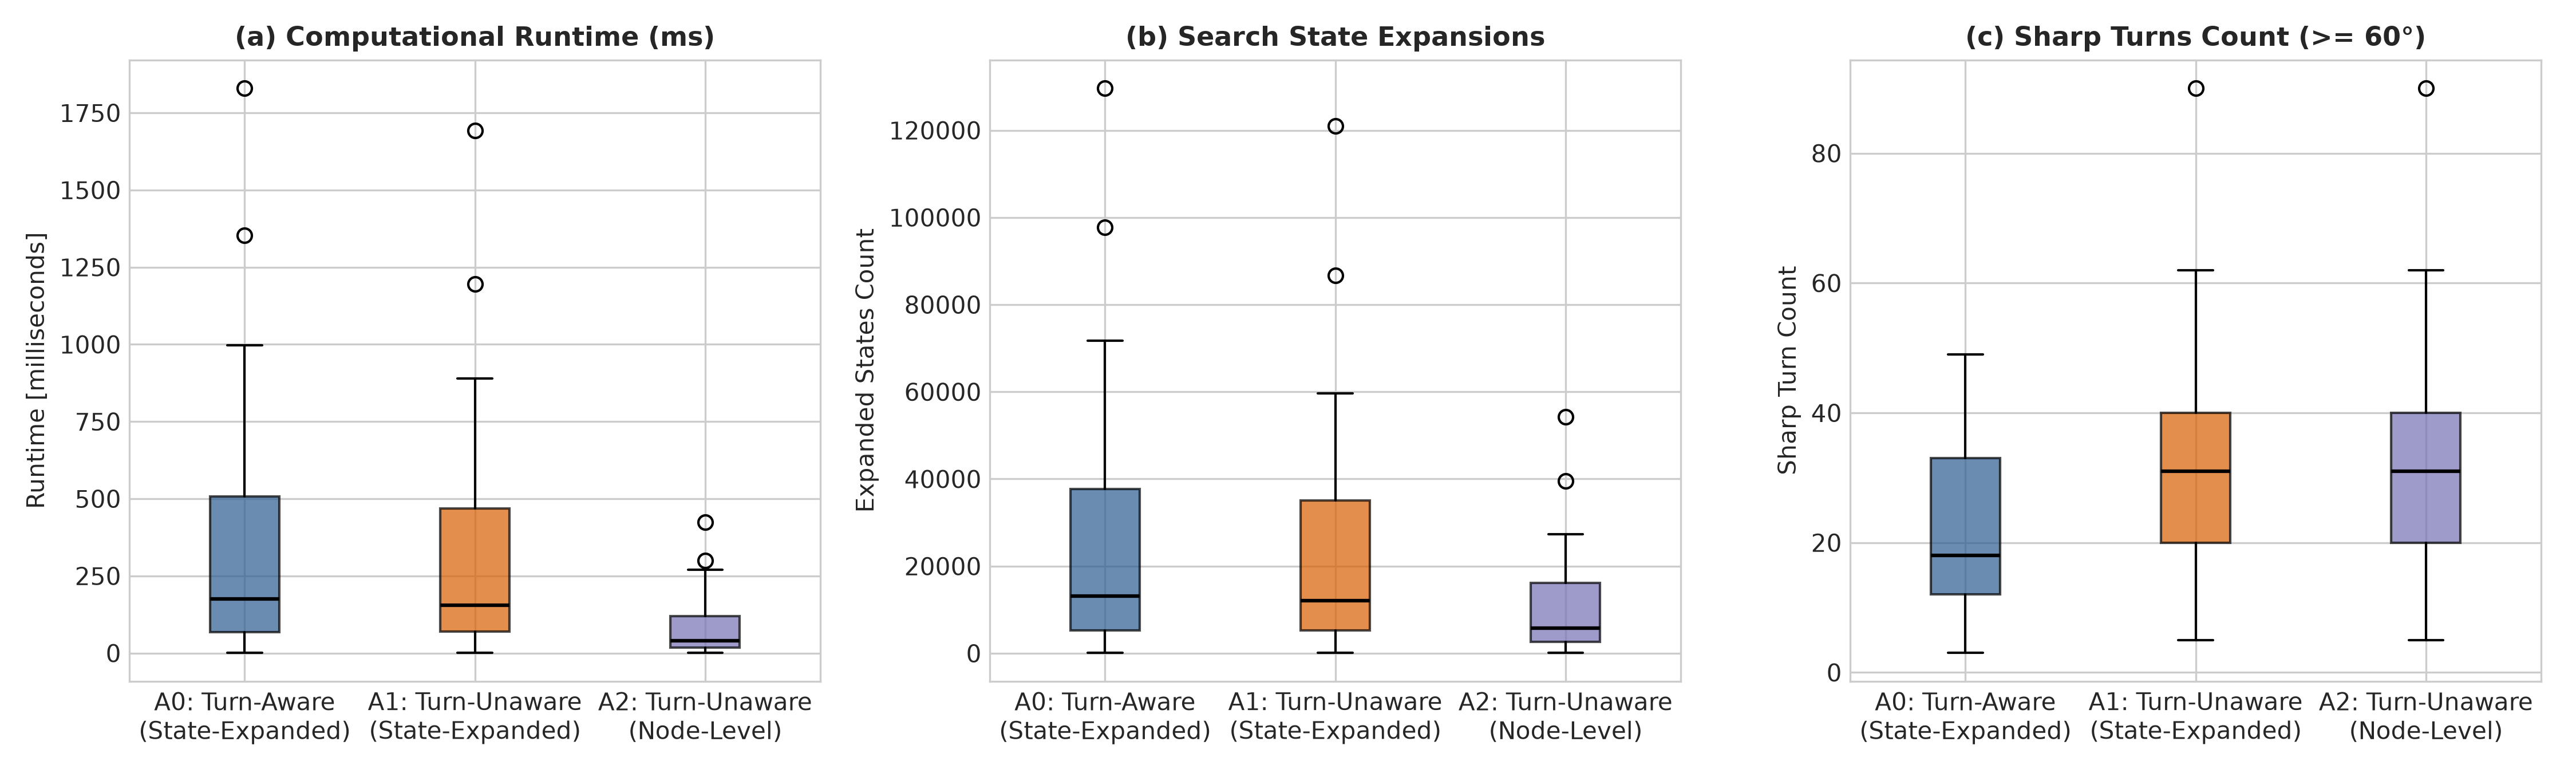
\includegraphics[width=\columnwidth]{fig1_exp_a_tradeoffs.png}
\caption{Experiment A routing trade-offs across 25 corridors: (a) sharp turns ($\ge 60^\circ$) under turn-aware ($A_0$) vs. turn-unaware state expansion ($A_1$) and node-level reference ($A_2$), (b) wall-clock runtime distributions (log scale), and (c) expanded states.}
\label{fig:exp_a_tradeoffs}
\end{figure}

\subsection{Road-Class Impedance and Street-Hierarchy Allocation}

Under production road impedance ($B_0$, Fig.~\ref{fig:exp_b_road_classes}), arterial exposure drops from $65.05\%$ under neutral weights ($B_1$) to $13.84\%$, a $51.21$ percentage-point reduction (Pratt $W = 4.0$, Holm $p_{\text{adj}} = 8.4 \times 10^{-5}$, Cohen's $d_z = -1.7715$, Hodges–Lehmann $-54.55\%$). Residential share expands from $13.51\%$ to $44.24\%$ ($+30.73$ percentage points, Pratt $W = 9.0$, Holm $p_{\text{adj}} = 1.5 \times 10^{-4}$, Cohen's $d_z = +1.5234$, Hodges–Lehmann $+31.30\%$). Arterial avoidance incurs a detour: $B_0$ paths average $7.647\text{ km}$ versus $6.620\text{ km}$ under $B_1$ ($+15.53\%$ or $+1.028\text{ km}$, Pratt $W = 7.0$, Holm $p_{\text{adj}} = 6.8 \times 10^{-5}$, Cohen's $d_z = +0.9246$, Hodges–Lehmann $+0.86\text{ km}$). Relative to physical shortest paths ($B_2$, $59.35\%$ arterial share), $B_0$ lowers arterial exposure by $45.51$ percentage points (Pratt $W = 4.0$, Holm $p_{\text{adj}} = 8.4 \times 10^{-5}$, Cohen's $d_z = -1.5862$, Hodges–Lehmann $-46.31\%$). Configured impedance scales edge traversal costs, distinct from physical distance or elapsed travel time.

\begin{figure}[t]
\centering
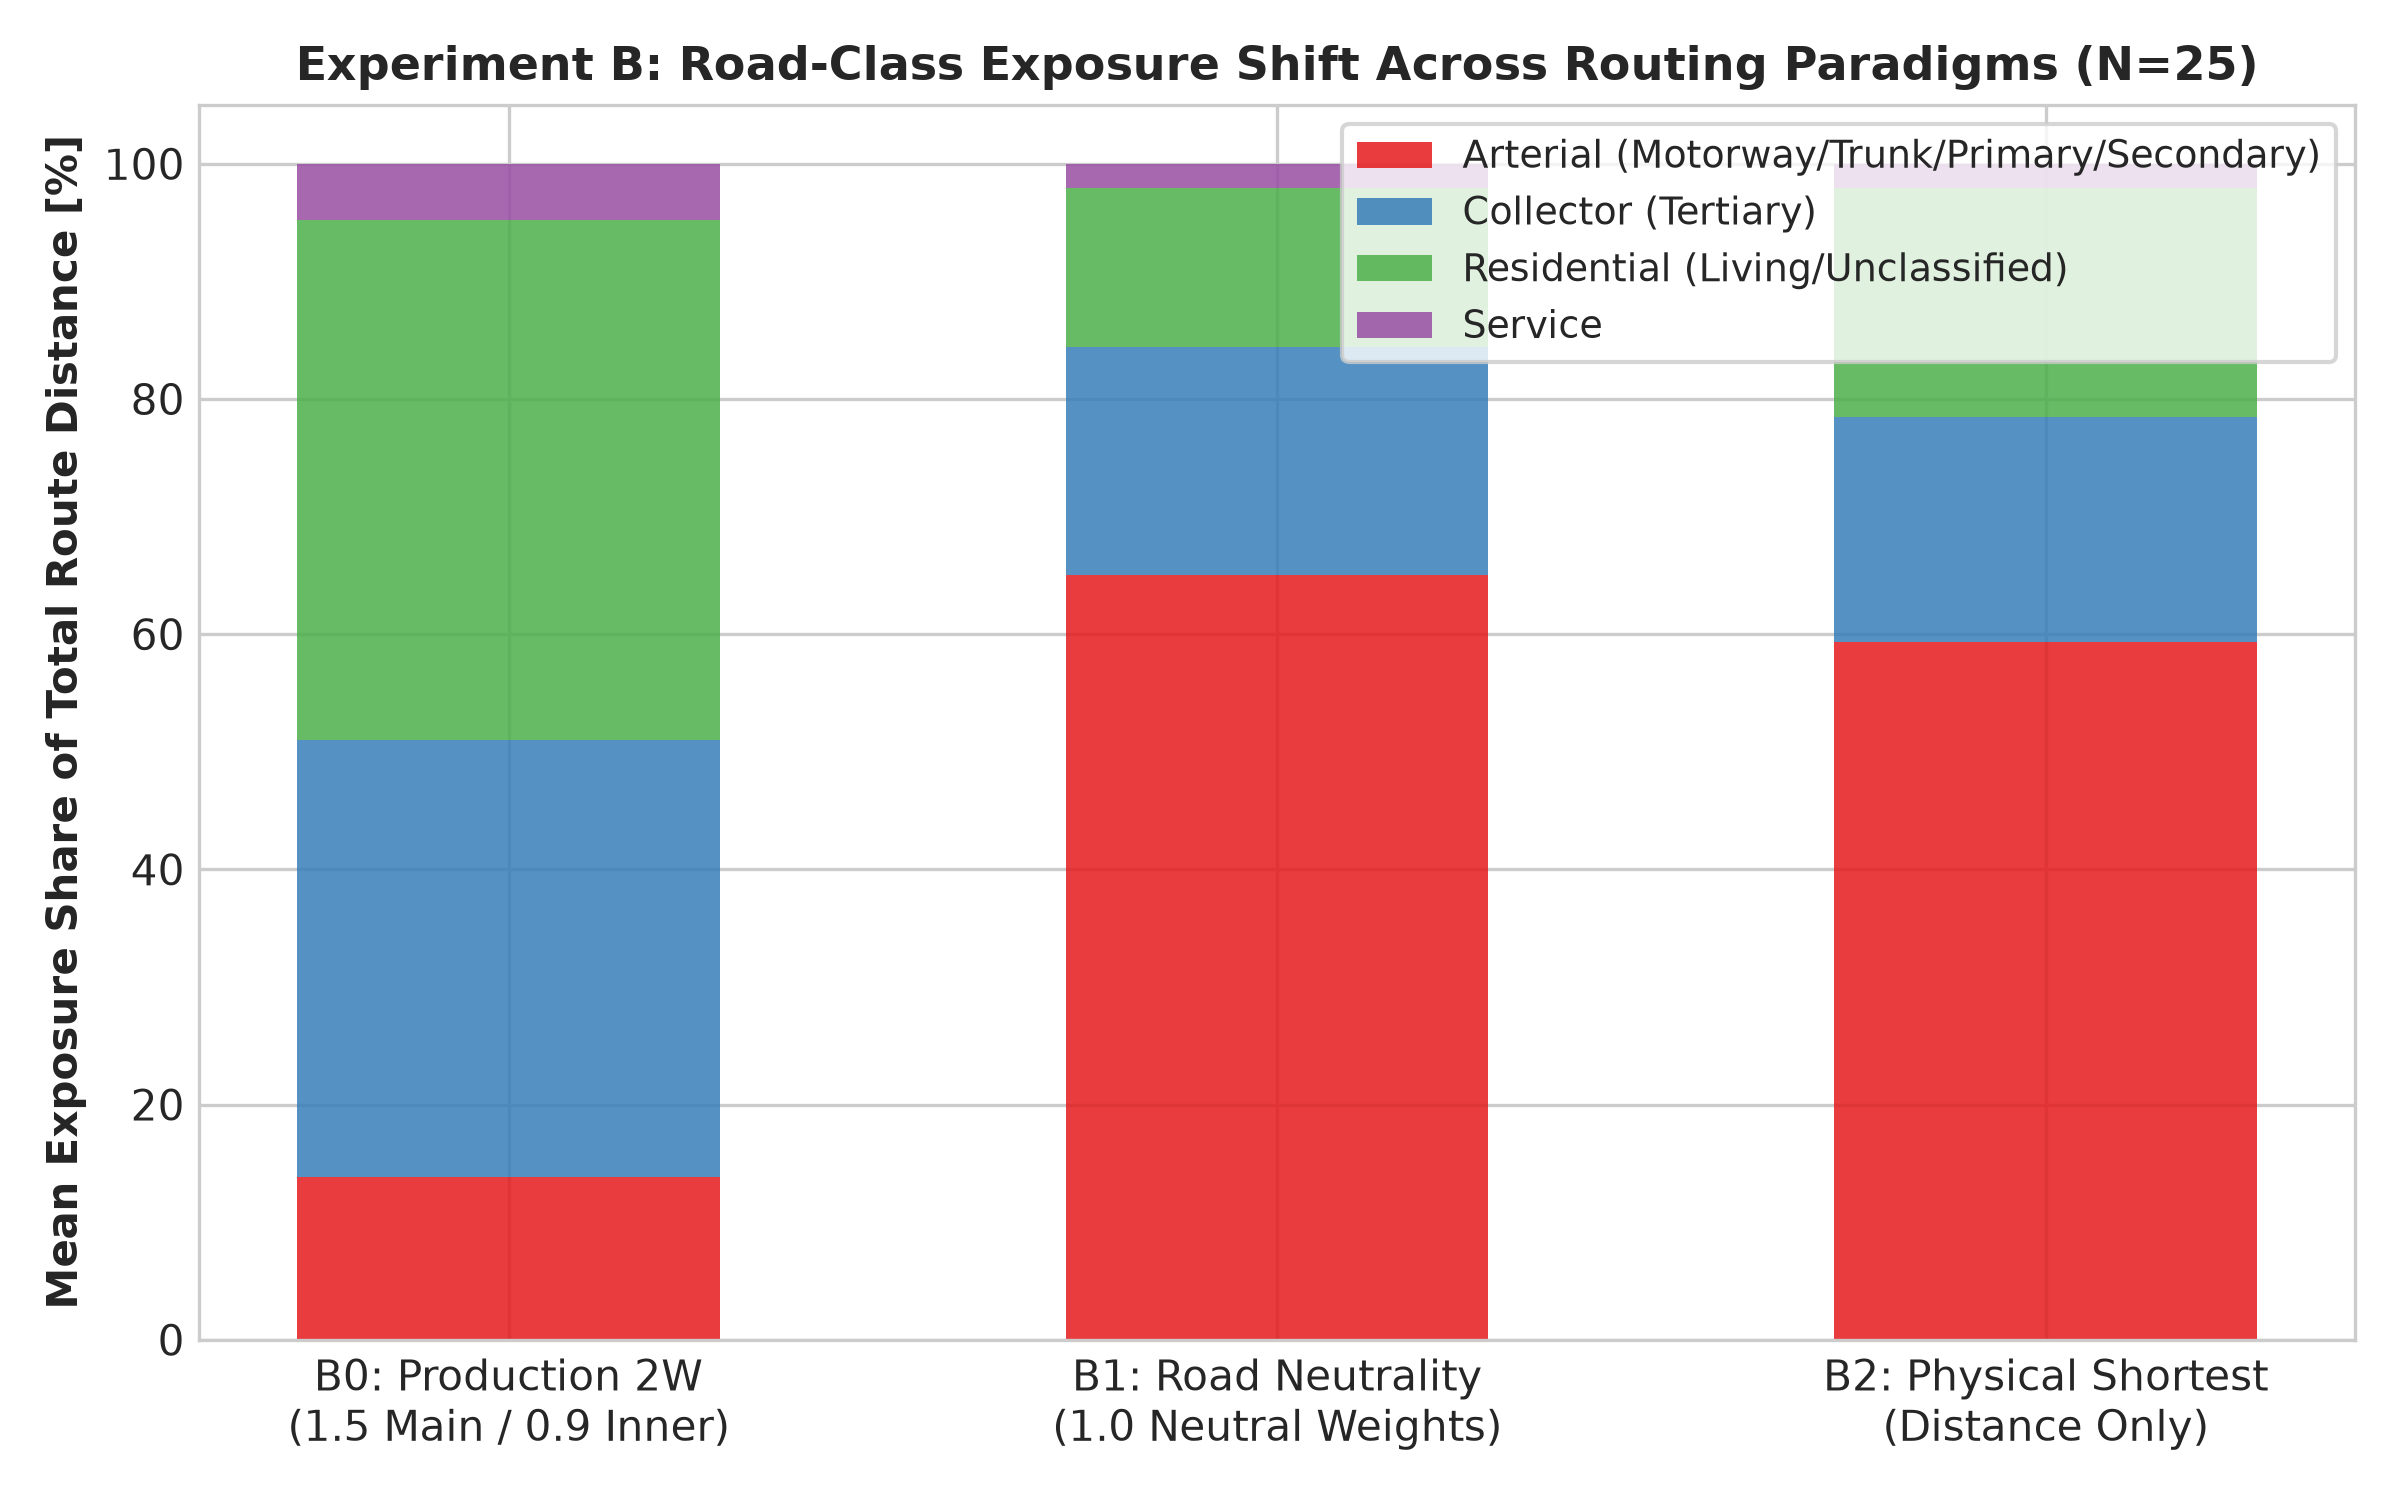
\includegraphics[width=\columnwidth]{fig2_exp_b_road_classes.png}
\caption{Experiment B street-hierarchy allocation across 25 corridors: (a) stacked percentage composition of road classes and (b) paired arterial versus residential street exposure shift across production ($B_0$), neutral ($B_1$), and shortest-distance ($B_2$) configurations.}
\label{fig:exp_b_road_classes}
\end{figure}

\subsection{Turn-Penalty Sensitivity and Empirical Trade-off Knee}

Across four penalty tiers (Fig.~\ref{fig:exp_c_sensitivity}), mean sharp turns decline monotonically: $C_0\ (0/0\text{ m}) = 32.52 \to C_1\ (12/4\text{ m}) = 24.64 \to C_2\ (25/8\text{ m}) = 21.44 \to C_3\ (50/16\text{ m}) = 19.80$ (pairwise tests vs. $C_2$: $p_{\text{adj}} \le 1.1 \times 10^{-4}$). Baseline $C_2$ captures $87.1\%$ of maximum turn reduction ($11.08 / 12.72$ turns) at minimum corpus mean distance ($7.648\text{ km}$). Escalating to $C_3$ shows diminishing returns: sharp turns decrease by only $1.64$ at $+32.3\text{ m}$ detour ($7.648 \to 7.680\text{ km}$, $+19.7\text{ m}$ per turn avoided; Pratt $W = 0.0$, Holm $p_{\text{adj}} = 1.1 \times 10^{-4}$, Cohen's $d_z = -1.0393$, Hodges–Lehmann $-1.50\text{ turns}$). Baseline $C_2$ represents an empirical trade-off knee rather than a universally dominant optimum: corridor breakdowns reveal that $C_2$ dominates $C_3$ on 8 corridors, $C_3$ dominates $C_2$ on 7, with 5 trade-offs and 5 ties.

\begin{figure}[t]
\centering
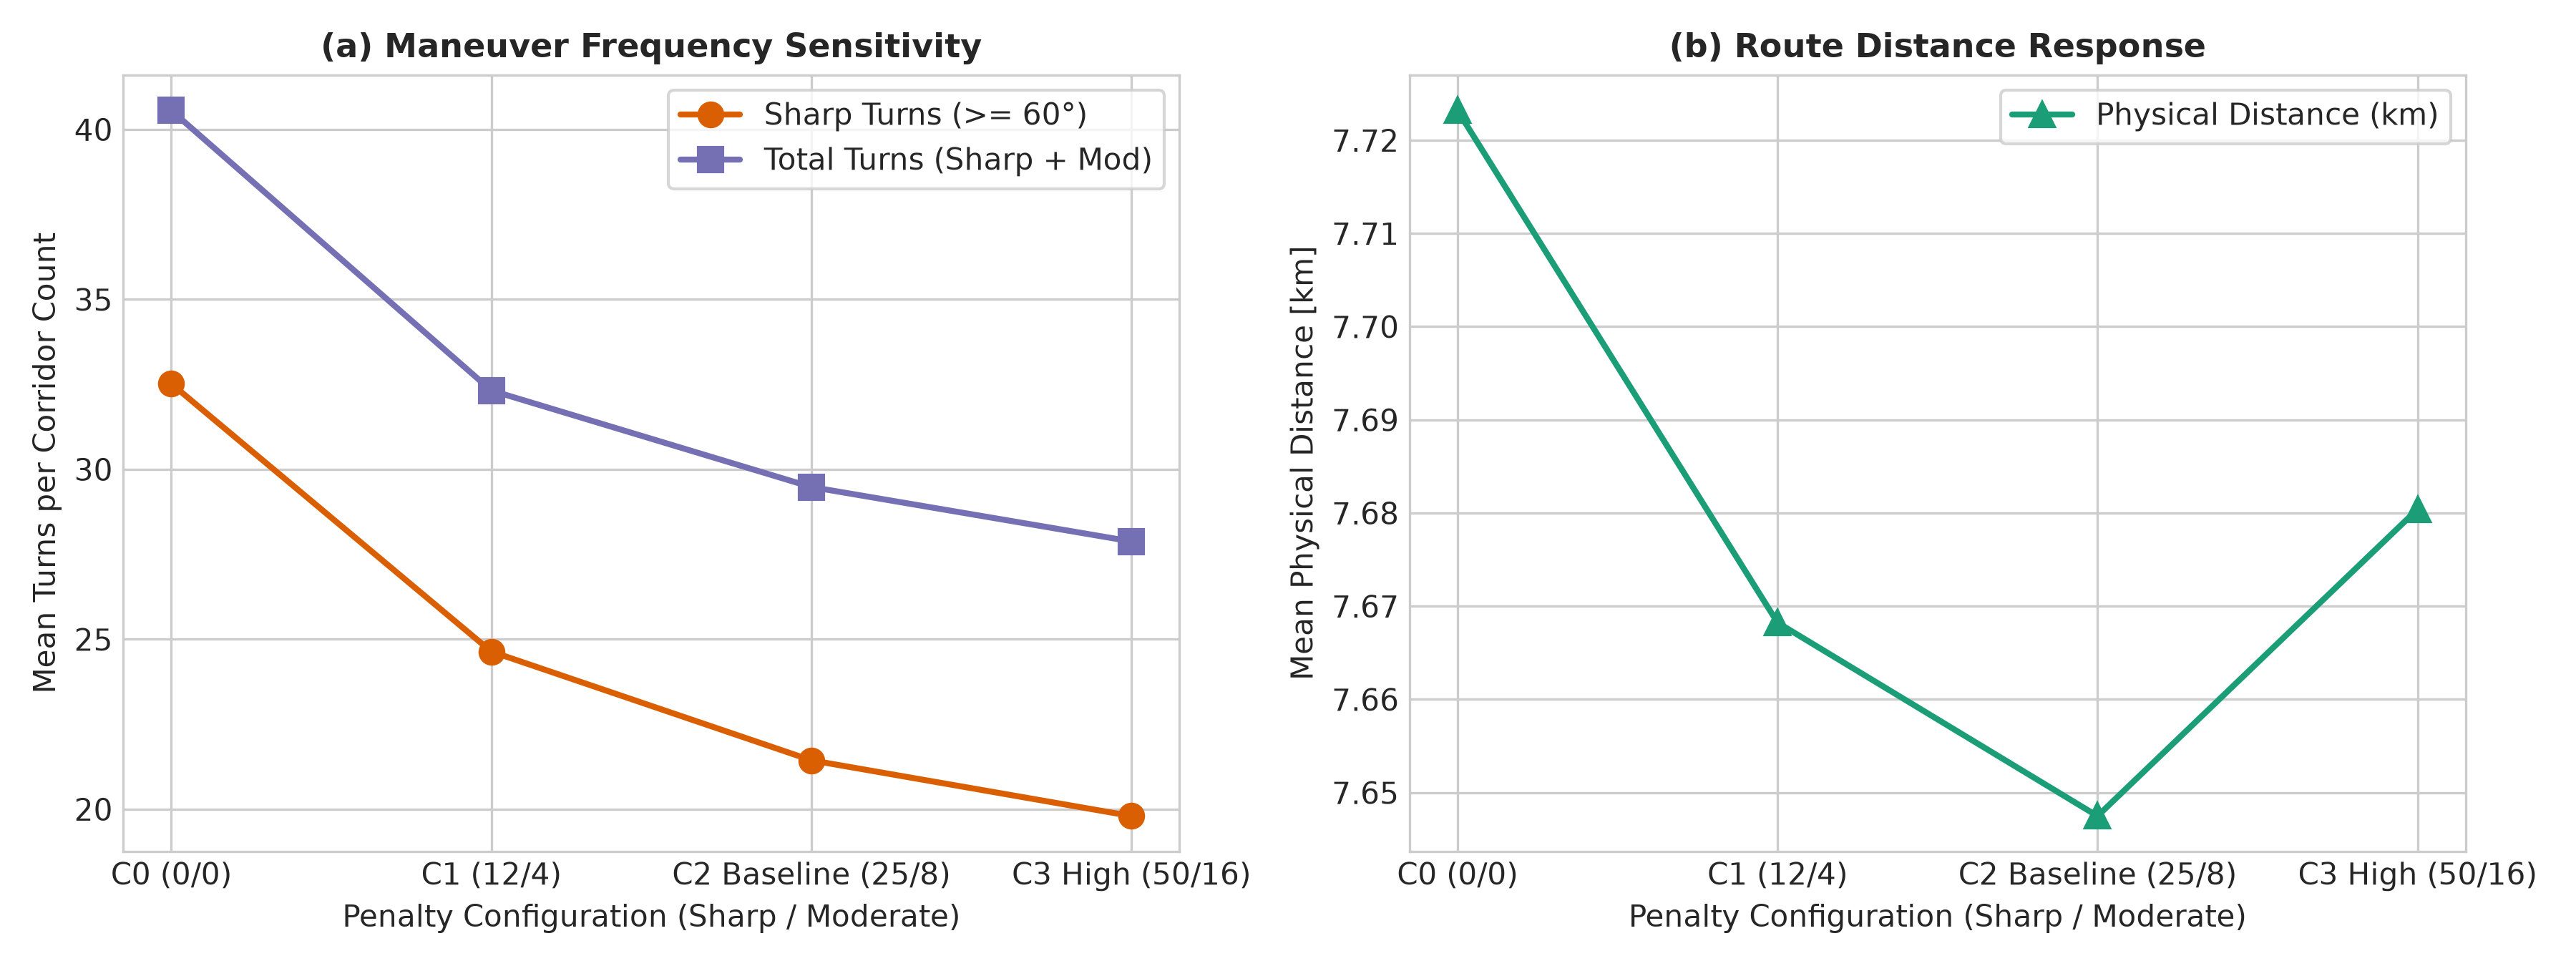
\includegraphics[width=\columnwidth]{fig3_exp_c_sensitivity.png}
\caption{Experiment C turn-penalty sensitivity across 25 corridors: (a) monotonic sharp turn reduction across tiers $C_0$ ($0/0\text{ m}$), $C_1$ ($12/4\text{ m}$), $C_2$ ($25/8\text{ m}$), and $C_3$ ($50/16\text{ m}$); (b) physical route distance versus sharp turns showing baseline $C_2$ as the empirical corpus-average trade-off knee.}
\label{fig:exp_c_sensitivity}
\end{figure}

\subsection{Topological Modifiers: Bridge and Roundabout Effects}

A $2 \times 2$ factorial design ($D_1\text{--}D_4$) tested bridge ($0.80$) and roundabout ($0.95$) modifiers. Bridge comparisons ($D_1$ vs. $D_2$, roundabout off; $D_3$ vs. $D_4$, roundabout on) shifted routes only on OD\_04 (approximately $-645\text{ m}$) and OD\_15 (approximately $-2.15\text{ km}$); 23 of 25 corridors were unchanged ($23/25$ zeros; Post-Hoc Standardized Impedance Cost $D_3$ vs. $D_4$: mean diff $+120.92$, $p_{\text{adj}} = 0.4722$, $d_z = +0.2192$). Roundabouts ($D_1$ vs. $D_3$, $D_2$ vs. $D_4$) produced zero route or distance changes ($25/25$ zeros; OD\_06 traversed $62.98\text{ m}$). Search-objective costs were not retained; post-hoc standardized production scoring yielded identical observed costs across corridors, with non-significant $D_2$ vs. $D_4$ testing ($p_{\text{adj}} = 1.000$, outside Table~\ref{tab:statistical_results}).

\subsection{Primary Inferential Hypothesis Test Summary}

Table~\ref{tab:statistical_results} summarizes the ten paired primary hypothesis tests across six families ($N=25$ corridors). Eight comparisons achieved statistical significance ($p_{\text{adj}} \le 1.5 \times 10^{-4}$); two were not statistically significant ($A_1$ vs. $A_2$ sharp turns, $p_{\text{adj}} = 1.000$; $D_3$ vs. $D_4$ Post-Hoc Standardized Impedance Cost, $p_{\text{adj}} = 0.4722$). Route-geometry and distance invariance ($25/25$ zeros for $A_1$ vs. $A_2$ and $D_2$ vs. $D_4$) represent separate descriptive findings.

\begin{table}[t]
\caption{Primary Paired Inferential Hypothesis Test Results ($N=25$ Corridors)}
\label{tab:statistical_results}
\centering
\footnotesize
\setlength{\tabcolsep}{2.2pt}
\begin{tabular}{llccc}
\hline
\textbf{Comparison} & \textbf{Outcome Metric} & \textbf{Mean Diff.} & \textbf{Wilcoxon $W$} & \textbf{Holm $p_{\mathrm{adj}}$} \\
\hline
$A_0$ vs $A_1$ & Sharp Turns ($\ge 60^\circ$) & $-11.08$ & $0.0$ & $\mathbf{4.5 \times 10^{-5}}$ \\
$A_1$ vs $A_2$ & Sharp Turns ($\ge 60^\circ$) & $0.00$ & $0.0$ & $1.000$ \\
$A_0$ vs $A_1$ & Wall-Clock Runtime [ms] & $+41.35$ & $17.0$ & $\mathbf{1.2 \times 10^{-5}}$ \\
$A_1$ vs $A_2$ & Wall-Clock Runtime [ms] & $+253.38$ & $0.0$ & $\mathbf{< 10^{-6}}$ \\
$B_0$ vs $B_1$ & Arterial Share [\%] & $-51.21$ & $4.0$ & $\mathbf{8.4 \times 10^{-5}}$ \\
$B_0$ vs $B_1$ & Residential Share [\%] & $+30.73$ & $9.0$ & $\mathbf{1.5 \times 10^{-4}}$ \\
$B_0$ vs $B_1$ & Physical Distance [km] & $+1.028$ & $7.0$ & $\mathbf{6.8 \times 10^{-5}}$ \\
$B_0$ vs $B_2$ & Arterial Share [\%] & $-45.51$ & $4.0$ & $\mathbf{8.4 \times 10^{-5}}$ \\
$C_3$ vs $C_2$ & Sharp Turns ($\ge 60^\circ$) & $-1.64$ & $0.0$ & $\mathbf{1.1 \times 10^{-4}}$ \\
$D_3$ vs $D_4$ & Post-Hoc Standardized Impedance Cost & $+120.92$ & $0.0$ & $0.4722$ \\
\hline
\multicolumn{5}{p{3.3in}}{\scriptsize \textit{Note:} Paired Wilcoxon signed-rank tests with Pratt zero-difference correction across $N=25$ OD corridors (8 significant, 2 non-significant). Bold values indicate statistical significance ($p_{\mathrm{adj}} < 0.05$). The $A_1$ vs. $A_2$ test strictly evaluates sharp-turn counts ($p_{\mathrm{adj}} = 1.000$); complete route-geometry and physical-distance invariance ($25/25$ zeros) are separate descriptive corridor-level findings. Metric label "Post-Hoc Standardized Impedance Cost" evaluates paths under restored standard production scoring; actual configured search-objective costs were not retained by the harness. Route-geometry and physical-distance invariance across all 25 corridors for the roundabout modifier ($D_2$ vs. $D_4$, $25/25$ zeros) are separate descriptive findings from corridor metrics detailed in Section~VI-D.}
\end{tabular}
\end{table}

\section{Conclusion and Future Work}

This study developed a state-expanded, turn-aware A* routing framework for two-wheeler routing on urban road networks. Directed edge states $s = (u, v)$ enable exact turn-cost evaluation without auxiliary path memory. Traversal costs are governed by road-class-dependent impedance modelling. Scaled by $\mu_{\min} = 0.80$, the Haversine heuristic is admissible and consistent under Theorem 1, conditioned on the lower bound $\mu(e) \ge 0.80$ verified on the evaluated Bengaluru graph.

Across 25 corridors, empirical ablations demonstrated marked routing shifts. Turn-aware search reduced sharp turns by $34.1\%$ relative to turn-unaware expansion ($p_{\text{adj}} = 4.5 \times 10^{-5}$) with median runtime increasing from $154.69$ to $174.93\text{ ms}$. Road-class impedance lowered arterial exposure by $51.21$ percentage points ($p_{\text{adj}} = 8.4 \times 10^{-5}$) with a $15.53\%$ increase in mean physical route distance ($p_{\text{adj}} = 6.8 \times 10^{-5}$). Configuration $C_2$ captured $87.1\%$ of the maximum observed turn reduction as an empirical corpus-average trade-off knee. Bridges shifted routes on two corridors (OD\_04 and OD\_15; 23 unchanged), while roundabouts produced zero geometric changes across all 25 corridors.

Methodological boundaries qualify these findings. Evaluations were restricted to Bengaluru's street network across 25 corridors. Lacking real-world journey-time measurements, travel-time reduction was not demonstrated; configured impedance scales algorithmic search costs, distinct from physical distance or travel time. Sharp-turn counts represent geometric manoeuvre measures and do not establish safety improvements or accident reduction. Multipliers lack behavioral rider calibration, and Experiment D search-objective costs were not retained.

Future work will evaluate the framework across diverse topologies to assess parameter transferability and heuristic bounds. Penalty weights will be calibrated using empirical GPS trajectories and rider choices. Collecting real-world journey times will evaluate whether the framework achieves its intended practical objective of time-efficient travel. Finally, incorporating dynamic traffic, gradients, and vehicle-specific constraints remains open.

\bibliographystyle{IEEEtran}
\bibliography{../paper1_literature/paper1_verified_references}

\end{document}
